\documentclass[11pt,a4paper]{article}
\usepackage[utf8]{inputenc}
\usepackage[margin=0.85in]{geometry}
\usepackage{amsmath,amssymb,amsfonts,amsthm}
\usepackage{tikz}
\usetikzlibrary{automata,positioning,arrows.meta,calc,shapes.geometric}
\usepackage{booktabs}
\usepackage{array}
\usepackage{xcolor}
\usepackage{tcolorbox}
\tcbuselibrary{skins,breakable}
\usepackage{enumitem}
\usepackage{hyperref}

% Color Palette
\definecolor{buetblue}{RGB}{0,51,102}
\definecolor{accentteal}{RGB}{0,128,128}
\definecolor{darkcrimson}{RGB}{139,0,0}
\definecolor{boxbg}{RGB}{246,249,253}
\definecolor{tablehead}{RGB}{225,236,248}

\hypersetup{
    colorlinks=true,
    linkcolor=buetblue,
    urlcolor=accentteal
}

% Custom Styled Callout Boxes
\newtcolorbox{questionbox}[2][]{
    enhanced,
    breakable,
    colback=boxbg,
    colframe=buetblue,
    coltitle=white,
    fonttitle=\bfseries,
    title={#2},
    attach boxed title to top left={yshift=-2mm, xshift=4mm},
    boxed title style={colback=buetblue},
    #1
}

\newtcolorbox{solutionbox}[1][]{
    enhanced,
    breakable,
    colback=white,
    colframe=accentteal,
    coltitle=white,
    fonttitle=\bfseries,
    title={Full Mathematical Solution \& Trace},
    attach boxed title to top left={yshift=-2mm, xshift=4mm},
    boxed title style={colback=accentteal},
    #1
}

\title{\textbf{\color{buetblue}CSE 211: Theory of Computation}\\
\large Complete Examination Solutions on Turing Machines \& Computability Theory}
\author{\textbf{Department of Computer Science and Engineering, BUET}}
\date{\today}

\begin{document}
\maketitle
\tableofcontents
\newpage

% ==============================================================================
% EXAM 2023-2024
% ==============================================================================
\part{Examination 2023--2024 (05/05/2026, 22-Batch)}

\section{Question 9: Binary Equality Comparator}
\begin{questionbox}{Question 9 (2023--24)}
Design a Turing machine (TM) that takes as input two numbers, $w_1$ and $w_2$, in binary, and determines whether the numbers are equal or not[cite: 4]. The tape initially contains $w_1 c w_2 c$ where `$c$' is a tape symbol that is used as a separator[cite: 4]. Your TM should compare $w_1$ and $w_2$, write 0 after the second $c$ if they are equal, and write 1 after the second $c$ otherwise[cite: 4]. (You can assume that the numbers are of the same length, and use multiple tracks and storage in the state if you wish)[cite: 4].
\end{questionbox}

\begin{solutionbox}
\textbf{1. Machine Strategy (2 Tracks \& State Storage):}
\begin{itemize}[leftmargin=*]
    \item \textbf{Track 1:} Checkmarks ($B$ for unchecked, $*$ for checked)[cite: 2].
    \item \textbf{Track 2:} Data characters ($0, 1, c, B$)[cite: 2].
    \item \textbf{State Storage:} $[q, \text{reg}]$ where $\text{reg} \in \{0, 1, B\}$ stores the bit transported from $w_1$ to compare against $w_2$[cite: 2].
\end{itemize}

\textbf{Detailed Algorithmic Flow:}
\begin{enumerate}[leftmargin=*]
    \item \textbf{Pick up Bit:} In state $[q_0,B]$, locate the leftmost unchecked symbol $a\in\{0,1\}$ of $w_1$, mark Track 1 with $*$, store $a$ in the finite control, and move right[cite: 2].
    \item \textbf{Seek $w_2$:} In state $[q_1,a]$, move right past the remaining symbols of $w_1$ and cross the first delimiter $c$ into state $[q_2,a]$[cite: 2].
    \item \textbf{Compare Bit:} In state $[q_2,a]$, skip previously checked symbols ($*$) of $w_2$[cite: 2]. At the first unchecked symbol $[B,b]$:
    \begin{itemize}
        \item If $b=a$, mark it checked, clear the register to $B$, and enter $q_{\text{rewind}}$ moving left[cite: 2].
        \item If $b\ne a$, a mismatch has been found; move to the blank after the second $c$, write \textbf{1}, and halt[cite: 2].
    \end{itemize}
    \item \textbf{Rewind:} Move left across $w_2$, the separator, and $w_1$ until the next unchecked position of $w_1$ can be reached; then return to $[q_0,B]$[cite: 2].
    \item \textbf{Equality Verification:} If $[q_0,B]$ encounters the first $c$, every bit of $w_1$ has already been matched with the corresponding bit of $w_2$. Move to the blank after the second $c$, write \textbf{0}, and halt[cite: 2].
\end{enumerate}

\textbf{2. Formal 7-Tuple:}
$$M = (Q, \Sigma, \Gamma, \delta, [q_0, B], [B, B], \{[q_{\text{halt}}, B]\}) \text{[cite: 2]}$$
where $\Sigma = \{[B, 0], [B, 1], [B, c]\}$ and $\Gamma = \{B, *\} \times \{0, 1, c, B\}$[cite: 2].

A more explicit state-set description is
$$Q = \{q_0,q_1,q_2,q_{\text{rewind}},q_{\text{scan}},q_{\text{mismatch}},q_{\text{write0}},q_{\text{write1}},q_{\text{halt}}\}\times\{0,1,B\}\text{[cite: 2]}.$$

\textbf{3. Transition Function $\delta$:} Let $a, b \in \{0, 1\}$.
\begin{center}
\small
\begin{tabular}{llll}
\toprule
\textbf{State} & \textbf{Scanned} & \textbf{Next State} & \textbf{Action} \\
\midrule
$[q_0, B]$ & $[B, a]$ & $[q_1, a]$ & Write $[*, a]$, Move $R$ (Pick bit from $w_1$)[cite: 2] \\
$[q_0, B]$ & $[B, c]$ & $[q_{\text{write0}}, B]$ & Write $[B, c]$, Move $R$ (All bits matched!)[cite: 2] \\
$[q_1, a]$ & $[B, 0/1]$ & $[q_1, a]$ & Write $[B, 0/1]$, Move $R$ (Scan across $w_1$)[cite: 2] \\
$[q_1, a]$ & $[B, c]$ & $[q_2, a]$ & Write $[B, c]$, Move $R$ (Enter $w_2$)[cite: 2] \\
$[q_2, a]$ & $[*, 0/1]$ & $[q_2, a]$ & Write $[*, 0/1]$, Move $R$ (Skip checked bits)[cite: 2] \\
$[q_2, a]$ & $[B, a]$ & $[q_{\text{rewind}}, B]$ & Write $[*, a]$, Move $L$ (\textbf{Match!})[cite: 2] \\
$[q_2, a]$ & $[B, \bar{a}]$ & $[q_{\text{write1}}, B]$ & Write $[*, \bar{a}]$, Move $R$ (\textbf{Mismatch!})[cite: 2] \\
$[q_{\text{rewind}}, B]$ & $[*, 0/1]$ or $[B, \text{any}]$ & $[q_{\text{rewind}}, B]$ & Move $L$ until reaching left boundary[cite: 2] \\
$[q_{\text{rewind}}, B]$ & (hit left boundary) & $[q_0, B]$ & Step $R$ to leftmost unchecked bit[cite: 2] \\
$[q_{\text{write0}}, B]$ & $[B/*, 0/1/c]$ & $[q_{\text{write0}}, B]$ & Move $R$ past second $c$[cite: 2] \\
$[q_{\text{write0}}, B]$ & $[B, B]$ & $[q_{\text{halt}}, B]$ & Write $[B, 0]$, Move $R$ (HALT)[cite: 2] \\
$[q_{\text{write1}}, B]$ & $[B/*, 0/1/c]$ & $[q_{\text{write1}}, B]$ & Move $R$ past second $c$[cite: 2] \\
$[q_{\text{write1}}, B]$ & $[B, B]$ & $[q_{\text{halt}}, B]$ & Write $[B, 1]$, Move $R$ (HALT)[cite: 2] \\
\bottomrule
\end{tabular}
\end{center}

\textbf{4. Trace for $w_1 = 10, w_2 = 10$ ($10c10c$):}
\begin{align*}
& [q_0, B]\,[B,1][B,0][B,c][B,1][B,0][B,c] \vdash [*,1]\,[q_1, 1]\,[B,0][B,c][B,1][B,0][B,c] \text{[cite: 2]} \\
& \vdash^* [*,1][B,0][B,c]\,[q_2, 1]\,[B,1][B,0][B,c] \vdash [*,1][B,0]\,[q_{\text{rewind}}, B]\,[B,c][*,1][B,0][B,c] \text{[cite: 2]} \\
& \vdash^* [*,1]\,[q_0, B]\,[B,0][B,c][*,1][B,0][B,c] \vdash [*,1][*,0]\,[q_1, 0]\,[B,c][*,1][B,0][B,c] \text{[cite: 2]} \\
& \vdash^* [*,1][*,0][B,c][*,1]\,[q_2, 0]\,[B,0][B,c] \vdash [*,1][*,0][B,c]\,[q_{\text{rewind}}, B]\,[*,1][*,0][B,c] \text{[cite: 2]} \\
& \vdash^* [*,1][*,0]\,[q_0, B]\,[B,c][*,1][*,0][B,c] \vdash [*,1][*,0][B,c]\,[q_{\text{write0}}, B]\,[*,1][*,0][B,c] \text{[cite: 2]} \\
& \vdash^* [*,1][*,0][B,c][*,1][*,0][B,c][B,0]\,[q_{\text{halt}}, B]\,[B,B] \quad \text{\textbf{(Appends 0 and Halts)}} \text{[cite: 2]}
\end{align*}
\end{solutionbox}

\section{Question 10: Multi-tape TM \& Single-Tape Simulation}
\begin{questionbox}{Question 10 (2023--24)}
What is a multi-tape Turing machine[cite: 4]? Explain how a one-tape Turing machine with multiple tracks and storage in the state can simulate a multi-tape Turing machine[cite: 4].
\end{questionbox}

\begin{solutionbox}
\textbf{1. Definition of Multi-tape TM:}
A Multi-tape TM consists of a single finite control with $k$ separate, independent physical tapes[cite: 3]. Each tape $i$ has its own independent read/write head[cite: 3]. In one move, based on current state $q$ and the $k$-tuple of scanned characters $(X_1, \dots, X_k)$, it:
1. Enters a new state $p$[cite: 3].
2. Overwrites each cell under each head with $Y_i$[cite: 3].
3. Moves each head independently in direction $D_i \in \{L, R, S\}$[cite: 3].
$$\delta: Q \times \Gamma^k \rightarrow Q \times \Gamma^k \times \{L, R, S\}^k \text{[cite: 3]}$$

\textbf{2. Simulation Construction (2k Tracks):}
Let $M$ be a $k$-tape TM. We build an equivalent 1-tape TM $N$ whose tape contains $2k$ tracks[cite: 3]:
\begin{itemize}[leftmargin=*]
    \item \textbf{Track $2i$:} Contains the content of tape $i$ of $M$[cite: 3].
    \item \textbf{Track $2i-1$:} Contains blanks everywhere except an asterisk ($*$) indicating the head position of tape $i$[cite: 3].
\end{itemize}

\textbf{3. Simulation of One Move of $M$:}
\begin{enumerate}[leftmargin=*]
    \item \textbf{Scan Phase:} $N$'s single head sweeps from the leftmost head marker to the rightmost head marker[cite: 3]. $N$'s finite control stores a tuple $[q, X_1, X_2, \dots, X_k, \text{count}]$, recording the symbol $X_i$ beneath each marker $*$, and counting markers so it knows when all $k$ symbols are collected[cite: 3].
    \item \textbf{Update Phase:} $N$ determines $M$'s move: $\delta(q, X_1, \dots, X_k) = (p, [Y_1, \dots, Y_k], [D_1, \dots, D_k])$[cite: 3]. $N$ sweeps back across the tracks, rewrites each cell $X_i$ with $Y_i$, and shifts the head marker $*$ on Track $2i-1$ left or right according to $D_i$[cite: 3].
    \item \textbf{State Update:} $N$ changes its internal control state to $p$[cite: 3].
\end{enumerate}
\textbf{Time Complexity:} After $n$ moves, the markers are separated by at most $2n$ cells[cite: 3]. The sweep takes $O(n)$ steps per move[cite: 3]. Simulating $n$ steps takes $\sum_{i=1}^n O(i) = O(n^2)$ time on a single tape[cite: 3].
\end{solutionbox}

\section{Question 11: Non-RE Language \& Halting Problem Undecidability}
\begin{questionbox}{Question 11 (2023--24)}
Provide an example of a language which is not recursively enumerable[cite: 4]. Devise a proof to show that the Halting problem is not recursive[cite: 4]. (You can assume that the Universal language is known to be not recursive)[cite: 4].
\end{questionbox}

\begin{solutionbox}
\textbf{1. Example of Non-RE Language:}
The \textbf{Diagonalization Language} ($L_d$) is not RE[cite: 5]:
$$L_d = \{w_i \mid w_i \notin L(M_i)\}$$
where $w_i$ is the $i$-th binary string and $M_i$ is the $i$-th Turing machine in lexicographical order.

\textbf{2. Proof that Halting Problem ($H_{\text{TM}}$) is Not Recursive:}
Assume $L_u = \{\langle M, w \rangle \mid M \text{ accepts } w\}$ is known to be non-recursive (undecidable)[cite: 4].
We define the Halting Problem:
$$H_{\text{TM}} = \{\langle M, w \rangle \mid M \text{ halts on input } w\} \text{[cite: 5]}$$

\textbf{Reduction ($L_u \le_m H_{\text{TM}}$):}
Suppose for contradiction that $H_{\text{TM}}$ is recursive[cite: 4]. Then there exists a decider $R$ such that:
$$R(\langle M, w \rangle) = \begin{cases} \text{ACCEPT} & \text{if } M \text{ halts on } w \\ \text{REJECT} & \text{if } M \text{ loops on } w \end{cases}$$
We construct a decider $D$ for $L_u$ using $R$ as a subroutine:
\begin{enumerate}[leftmargin=*]
    \item On input $\langle M, w \rangle$, run decider $R$ on $\langle M, w \rangle$.
    \item If $R$ rejects, then $M$ loops forever on $w$; therefore $M$ cannot accept $w$. Decider $D$ \textbf{REJECTS}.
    \item If $R$ accepts, then $M$ is guaranteed to halt on $w$. Run the universal simulation of $M$ on $w$ until it terminates.
    \item If $M$ enters an accept state, $D$ \textbf{ACCEPTS}; otherwise, $D$ \textbf{REJECTS}.
\end{enumerate}
Decider $D$ halts on all inputs and decides $L_u$, contradicting that $L_u$ is non-recursive[cite: 4]. Thus, the Halting Problem is not recursive (undecidable)[cite: 4].
\end{solutionbox}

\section{Question 12: Complexity Hierarchy \& PSPACE vs. NPSPACE}
\begin{questionbox}{Question 12 (2023--24)}
i) Draw a Venn diagram showing the widely believed relationship among the classes of languages P, NP, NP-complete, recursive, and recursively enumerable[cite: 4]. \\
ii) What is the relationship between the classes PSPACE and NPSPACE[cite: 4]? Justify your answer briefly[cite: 4].
\end{questionbox}

\begin{solutionbox}
\textbf{1. Venn Diagram of Complexity Classes:}
\begin{center}
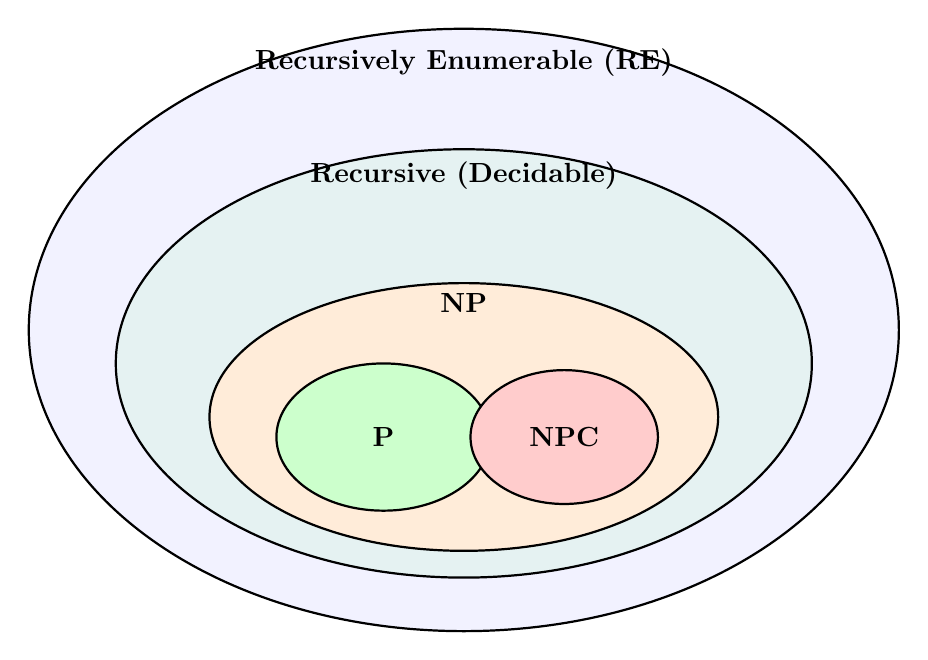
\begin{tikzpicture}[scale=0.85]
    % RE
    \draw[thick, fill=blue!5] (0,0) ellipse (6.5cm and 4.5cm);
    \node at (0, 4.0) {\textbf{Recursively Enumerable (RE)}};
    
    % Recursive
    \draw[thick, fill=teal!10] (0,-0.5) ellipse (5.2cm and 3.2cm);
    \node at (0, 2.3) {\textbf{Recursive (Decidable)}};
    
    % NP
    \draw[thick, fill=orange!15] (0,-1.3) ellipse (3.8cm and 2.0cm);
    \node at (0, 0.4) {\textbf{NP}};
    
    % P
    \draw[thick, fill=green!20] (-1.2,-1.6) ellipse (1.6cm and 1.1cm);
    \node at (-1.2, -1.6) {\textbf{P}};
    
    % NP-Complete
    \draw[thick, fill=red!20] (1.5,-1.6) ellipse (1.4cm and 1.0cm);
    \node at (1.5, -1.6) {\textbf{NPC}};
\end{tikzpicture}
\end{center}

\textbf{2. Relationship between PSPACE and NPSPACE:}
$$\mathbf{PSPACE = NPSPACE}$$
\textbf{Justification (Savitch's Theorem):} Savitch's Theorem states that for any space-constructible function $f(n) \ge \log n$, $\text{NSPACE}(f(n)) \subseteq \text{DSPACE}((f(n))^2)$. For polynomial space, $f(n) = n^k$. Therefore:
$$\text{NPSPACE} \subseteq \text{DSPACE}((n^k)^2) = \text{DSPACE}(n^{2k}) \subseteq \text{PSPACE}$$
Since deterministic space is trivially a subset of nondeterministic space ($\text{PSPACE} \subseteq \text{NPSPACE}$), they are identical: $\mathbf{PSPACE = NPSPACE}$.
\end{solutionbox}

\section{Question 13: Cook's Theorem \& Local Transition Formula}
\begin{questionbox}{Question 13 (2023--24)}
Briefly explain how Cook's theorem shows that all problems in NP are reducible to the satisfiability problem[cite: 4]. Suppose, a non-deterministic Turing machine has a transition rule $\delta(q, t) = \{(q_1, t_1, R), (q_2, t_2, L)\}$[cite: 4]. Construct the corresponding rule in the Boolean satisfiability formula according to Cook's construction if the tape head is at the $i$-th cell in the $j$-th step[cite: 4].
\end{questionbox}

\begin{solutionbox}
\textbf{1. Cook's Theorem Explanation:}
Cook's Theorem proves SAT is NP-complete by showing that for \textit{any} language $L \in \text{NP}$, an input $w$ can be converted in polynomial time into a Boolean formula $\Phi_{M, w}$ that is satisfiable if and only if the polynomial-time NTM $M$ accepts $w$. The formula uses Boolean variables representing:
1. $P[i, k]$: Tape cell $i$ contains symbol $X_k$ at time step $j$.
2. $Q[j, q]$: NTM is in state $q$ at step $j$.
3. $H[j, i]$: Head is scanning cell $i$ at step $j$.
Valid configurations and transitions are encoded as local CNF clauses enforcing initial state, head movement, valid transitions, and reachability of $q_{\text{accept}}$.

\textbf{2. Constructing the Transition Rule Formula:}
At step $j$, the tape head is at cell $i$, scanning symbol $t$ in state $q$. The premise condition is:
$$\text{Premise} = Q[j, q] \land H[j, i] \land P[j, i, t]$$
The rule allows two choices: $(q_1, t_1, R)$ OR $(q_2, t_2, L)$[cite: 4]. Therefore, at step $j+1$, the formula enforces:
$$\text{Premise} \implies \left( \begin{aligned}
& (Q[j+1, q_1] \land P[j+1, i, t_1] \land H[j+1, i+1]) \\
& \lor (Q[j+1, q_2] \land P[j+1, i, t_2] \land H[j+1, i-1])
\end{aligned} \right)$$
In CNF format, using the equivalence $(A \implies B_1 \lor B_2) \equiv (\neg A \lor B_1 \lor B_2)$:
$$(\neg Q[j, q] \lor \neg H[j, i] \lor \neg P[j, i, t]) \lor \left( \text{Choice}_1 \lor \text{Choice}_2 \right)$$
\end{solutionbox}

% ==============================================================================
% EXAM 2022-2023
% ==============================================================================
\part{Examination 2022--2023 (19/01/2025)}

\section{Question 10: Logical Bitwise NOT Appender}
\begin{questionbox}{Question 10 (2022--23)}
Design a Turing machine (TM) that takes as input a number $w$ in binary and computes the logical NOT of the number. The tape initially contains $wc$ where `$c$' is a tape symbol that is used as a separator. Your TM should insert the NOT of the number in binary after the $c$ and then terminate. (You can use multiple tracks and storage in the state if you wish).
\end{questionbox}

\begin{solutionbox}
\textbf{Detailed Design Concept:}
For every unchecked bit $a\in\{0,1\}$ in $w$, the machine performs the following cycle[cite: 2]:
\begin{enumerate}[leftmargin=*]
    \item Read $a$, mark that input position with $*$ on Track 1, and load its complement $\bar a=1-a$ into the finite-control register[cite: 2].
    \item Move right past $c$ and all output bits already written until reaching the first blank cell $[B,B]$[cite: 2].
    \item Write $[B,\bar a]$, then rewind left to the next unchecked bit of $w$[cite: 2].
    \item When $c$ is encountered in the initial scanning state, every input bit has been inverted, so the machine halts[cite: 2].
\end{enumerate}

\textbf{1. Architecture:}
\begin{itemize}[leftmargin=*]
    \item Track 1 stores checkmarks ($B$ or $*$)[cite: 2].
    \item Track 2 stores data bits $\{0, 1, c, B\}$[cite: 2].
    \item States store $[q, \text{bit}]$ where $\text{bit} \in \{0, 1, B\}$[cite: 2].
\end{itemize}

\textbf{2. Transition Rules:}
\begin{align*}
\delta([q_0, B], [B, a]) &= ([q_{\text{seek}}, \bar{a}], [*, a], R) \quad \text{for } a \in \{0, 1\} \text{ (Store inverted bit } \bar{a}\text{)} \text{[cite: 2]} \\
\delta([q_{\text{seek}}, \bar{a}], [B/*, \text{any non-blank}]) &= ([q_{\text{seek}}, \bar{a}], \text{same}, R) \quad \text{(Scan to the blank at end)} \text{[cite: 2]} \\
\delta([q_{\text{seek}}, \bar{a}], [B, B]) &= ([q_{\text{rewind}}, B], [B, \bar{a}], L) \quad \text{(Append inverted bit)} \text{[cite: 2]} \\
\delta([q_{\text{rewind}}, B], \text{any}) &= ([q_{\text{rewind}}, B], \text{same}, L) \quad \text{(Rewind left to } * \text{)} \text{[cite: 2]} \\
\delta([q_{\text{rewind}}, B], \text{leftmost } *) &= ([q_0, B], \text{same}, R) \quad \text{(Step right to next bit)} \text{[cite: 2]} \\
\delta([q_0, B], [B, c]) &= ([q_{\text{halt}}, B], [B, c], S) \quad \text{(All bits inverted } \implies \text{HALT)} \text{[cite: 2]}
\end{align*}

\textbf{State Transition Diagram:}
\begin{center}
\begin{tikzpicture}[->, >=Stealth, auto, node distance=3.2cm, semithick]
    \node[state, initial] (q0) {$q_0$};
    \node[state] (q_trans) [right of=q0] {$q_{\text{write}}$};
    \node[state] (q_back) [below of=q_trans] {$q_{\text{rewind}}$};
    \node[state, accepting] (q_halt) [below of=q0] {$q_{\text{halt}}$};

    \path (q0) edge [bend left] node[above] {$[B,a]/[*,a],R\;\text{ (store }\bar a\text{)}$[cite: 2]} (q_trans)
               edge node[left] {$[B,c]/[B,c],S$[cite: 2]} (q_halt)
          (q_trans) edge [loop right] node[right, align=left] {$[B/*,0/1/c]/\\ \text{same},R$[cite: 2]} (q_trans)
                    edge node[right] {$[B,B]/[B,\bar a],L$[cite: 2]} (q_back)
          (q_back) edge [loop below] node[below] {$[B/*,\text{any}]/\text{same},L$[cite: 2]} (q_back)
                   edge [bend left] node[left] {hit $[*,\text{any}]\rightarrow$ step $R$[cite: 2]} (q0);
\end{tikzpicture}
\end{center}

\textbf{3. ID Trace for $w = 101$ ($101c \rightarrow 101c010$):}
\begin{align*}
[q_0, B]101c &\vdash * [q_{\text{seek}}, 0] 01c \vdash^* *01c [q_{\text{seek}}, 0] B \vdash *01 [q_{\text{rewind}}, B] c0 \text{[cite: 2]} \\
&\vdash^* * [q_0, B] 01c0 \vdash ** [q_{\text{seek}}, 1] 1c0 \vdash^* **1c0 [q_{\text{seek}}, 1] B \vdash **1c [q_{\text{rewind}}, B] 01 \text{[cite: 2]} \\
&\vdash^* ** [q_0, B] 1c01 \vdash *** [q_{\text{seek}}, 0] c01 \vdash^* ***c01 [q_{\text{seek}}, 0] B \vdash ***c0 [q_{\text{rewind}}, B] 10 \text{[cite: 2]} \\
&\vdash^* *** [q_0, B] c010 \vdash ***c [q_{\text{halt}}, B] 010 \quad \text{\textbf{(Terminated with 010 appended)}} \text{[cite: 2]}
\end{align*}
\end{solutionbox}

\section{Question 11: Polynomial Simulation Claims}
\begin{questionbox}{Question 11 (2022--23)}
Justify whether the following statements are true or false: \\
(i) A deterministic Turing machine can simulate $n$ moves of a conventional computer in $P(n)$ moves, where $P(n)$ is some polynomial in $n$[cite: 3]. \\
(ii) A conventional computer can simulate $n$ moves of a non-deterministic Turing machine in $P(n)$ moves, where $P(n)$ is some polynomial in $n$[cite: 3].
\end{questionbox}

\begin{solutionbox}
\textbf{(i) Statement 1 is TRUE[cite: 3].}
Under standard models of computers where single instructions cannot increase word length by more than 1 bit (preventing $O(1)$ unbounded multiplications):
\begin{itemize}[leftmargin=*]
    \item After $n$ steps, memory has at most $O(n)$ words of length $O(n)$, occupying $O(n^2)$ tape cells on a TM[cite: 3].
    \item Simulating one step takes $O(n^2)$ time on a multi-tape TM[cite: 3].
    \item $n$ steps take $O(n^3)$ on a multi-tape TM, and $O((n^3)^2) = O(n^6)$ on a single-tape TM[cite: 3].
    \item Since $O(n^6)$ is polynomial, a DTM simulates a computer in polynomial time[cite: 3].
\end{itemize}

\textbf{(ii) Statement 2 is FALSE[cite: 3].}
An NTM with branching factor $m \ge 2$ can reach up to $m^n$ distinct configurations in $n$ moves[cite: 3]. Simulating these on a deterministic computer requires exploring this exponential tree (e.g., via BFS), requiring $O(m^n)$ operations[cite: 3]. A polynomial-time simulation would imply $P = NP$, which is widely believed to be false.
\end{solutionbox}

\section{Question 12: Diagonalization Language Non-RE Proof}
\begin{questionbox}{Question 12 (2022--23)}
What is the Diagonalization language? Devise a proof to show that the Diagonalization language is not recursively enumerable.
\end{questionbox}

\begin{solutionbox}
\textbf{1. Definition:}
Let $w_1, w_2, \dots$ be the canonical enumeration of all binary strings, and $M_1, M_2, \dots$ be the enumeration of all Turing machines. The Diagonalization language is:
$$L_d = \{w_i \mid w_i \notin L(M_i)\}$$

\textbf{2. Proof that $L_d$ is not RE (By Contradiction):}
Suppose $L_d$ is Recursively Enumerable. Then there must exist some Turing Machine $M_k$ that accepts $L_d$, meaning $L(M_k) = L_d$.

Now, query whether the string $w_k$ (the $k$-th string corresponding to $M_k$) belongs to $L_d$:
\begin{itemize}[leftmargin=*]
    \item \textbf{Case 1: $w_k \in L_d$.}
    By definition of $L_d$, $w_k \in L_d \implies w_k \notin L(M_k)$. But since $L(M_k) = L_d$, this implies $w_k \notin L_d$, a contradiction.
    \item \textbf{Case 2: $w_k \notin L_d$.}
    By definition of $L_d$, $w_k \notin L_d \implies w_k \in L(M_k)$. But since $L(M_k) = L_d$, this implies $w_k \in L_d$, a contradiction.
\end{itemize}
In both cases, we arrive at $w_k \in L_d \iff w_k \notin L_d$. Thus, no such Turing machine $M_k$ can exist, proving $L_d$ is \textbf{not Recursively Enumerable}.
\end{solutionbox}

% ==============================================================================
% EXAM 2021-2022
% ==============================================================================
\part{Examination 2021--2022 (31/01/2023)}

\section{Question 9: Signed-Magnitude to Two's Complement}
\begin{questionbox}{Question 9 (2021--22)}
Construct a Turing machine that takes as input a number $w$ in signed magnitude form and computes the 2's complement of the number. Initially the tape contains a number in binary, MSB being the leftmost bit. If the MSB is 0, the number will remain the same. However, if the MSB is 1, $w$ needs to be converted to its two's complement. Recall that you can convert a number to its two's complement by working from the least significant bit (LSB) towards the most significant bit (MSB), copying all the zeros until the first 1 is reached; then copy that 1, and flipping all the remaining bits (leave the MSB as 1). Your TM should terminate with only the two's complement of the number on the tape.
\end{questionbox}

\begin{solutionbox}
\textbf{1. Transition Logic:}
\begin{itemize}[leftmargin=*]
    \item $q_0$: If scanned bit is $0$, halt immediately (positive number). If $1$, leave as $1$, enter $q_{\text{seek\_end}}$ moving $R$.
    \item $q_{\text{seek\_end}}$: Skip all $0$s and $1$s moving right until finding blank $B$. Step left into $q_{\text{copy\_zeros}}$ (now at LSB).
    \item $q_{\text{copy\_zeros}}$: Moving left, leave all $0$s unchanged until the first $1$ is read. Leave that $1$ unchanged and enter $q_{\text{flip}}$ moving left.
    \item $q_{\text{flip}}$: Moving left, invert every bit ($0 \rightarrow 1$ and $1 \rightarrow 0$) until reaching the MSB cell.
    \item $q_{\text{halt}}$: Halt.
\end{itemize}

\textbf{2. Transition Table:}
\begin{center}
\small
\begin{tabular}{lllll}
\toprule
\textbf{State} & \textbf{Input 0} & \textbf{Input 1} & \textbf{Input B} & \textbf{Notes} \\
\midrule
$q_0$ & $(q_{\text{halt}}, 0, S)$ & $(q_{\text{seek}}, 1, R)$ & — & Check sign bit \\
$q_{\text{seek}}$ & $(q_{\text{seek}}, 0, R)$ & $(q_{\text{seek}}, 1, R)$ & $(q_{\text{copy}}, B, L)$ & Seek to LSB \\
$q_{\text{copy}}$ & $(q_{\text{copy}}, 0, L)$ & $(q_{\text{flip}}, 1, L)$ & $(q_{\text{halt}}, B, R)$ & Copy trailing zeros until first 1 \\
$q_{\text{flip}}$ & $(q_{\text{flip}}, 1, L)$ & $(q_{\text{flip}}, 0, L)$ & $(q_{\text{halt}}, B, R)$ & Invert remaining bits \\
\bottomrule
\end{tabular}
\end{center}

\textbf{3. State Diagram:}
\begin{center}
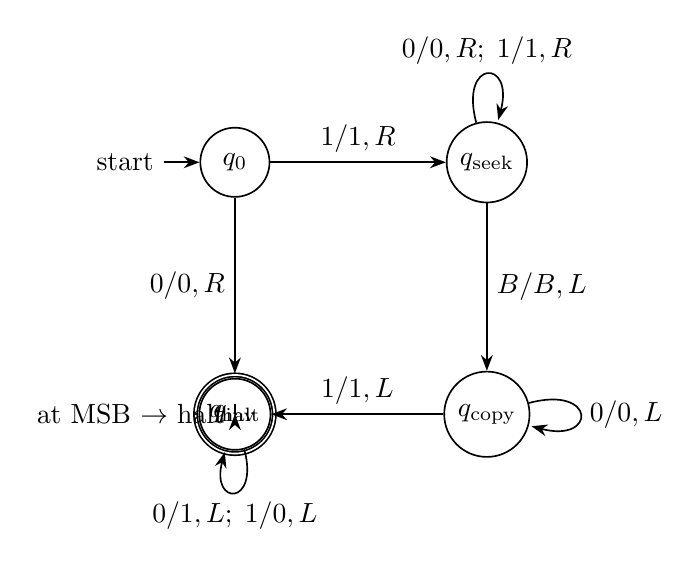
\begin{tikzpicture}[->, >=Stealth, auto, node distance=3.2cm, semithick]
    \node[state, initial] (q0) {$q_0$};
    \node[state] (q_seek) [right of=q0] {$q_{\text{seek}}$};
    \node[state] (q_copy) [below of=q_seek] {$q_{\text{copy}}$};
    \node[state] (q_inv) [left of=q_copy] {$q_{\text{inv}}$};
    \node[state, accepting] (q_halt) [below of=q0] {$q_{\text{halt}}$};

    \path (q0) edge node[above] {$1/1,R$} (q_seek)
               edge node[left] {$0/0,R$} (q_halt)
          (q_seek) edge [loop above] node[above] {$0/0,R;\;1/1,R$} (q_seek)
                   edge node[right] {$B/B,L$} (q_copy)
          (q_copy) edge [loop right] node[right] {$0/0,L$} (q_copy)
                   edge node[above] {$1/1,L$} (q_inv)
          (q_inv) edge [loop below] node[below] {$0/1,L;\;1/0,L$} (q_inv)
                  edge node[left] {at MSB $\rightarrow$ halt} (q_halt);
\end{tikzpicture}
\end{center}

\textbf{4. Trace on Input $11100$ (Negative Value):}
The magnitude part is $1100$. Moving from the LSB, copy the trailing $00$, copy the first $1$, and invert the remaining magnitude bit; the final tape is $10100$.
$$
\begin{array}{rll}
q_0 11100 & \vdash 1q_{\text{seek}}1100 \vdash^* 11100q_{\text{seek}}B & \text{(Seek to end)} \\
& \vdash 1110q_{\text{copy}}0 & \text{(At LSB)} \\
& \vdash 111q_{\text{copy}}00 & \text{(Copy trailing zero)} \\
& \vdash 11q_{\text{inv}}100 & \text{(First 1 copied; switch to invert)} \\
& \vdash 1q_{\text{inv}}0100 & \text{(Invert the remaining magnitude bit)} \\
& \vdash q_{\text{halt}}10100 & \textbf{(Preserve MSB 1 and HALT)}
\end{array}
$$
\end{solutionbox}

\section{Question 10: Multitrack Simulation \& NTM Complexity}
\begin{questionbox}{Question 10 (2021--22)}
Justify whether the following statements are true or false: \\
i) A one-tape Turing machine with multiple tracks can simulate a Multi-tape Turing machine[cite: 3]. \\
ii) A conventional computer can simulate $n$ moves of a non-deterministic Turing machine in $P(n)$ moves, where $P(n)$ is some polynomial in $n$[cite: 3].
\end{questionbox}

\begin{solutionbox}
\textbf{i) Statement 1 is TRUE[cite: 3].} As proven in Lecture 6, a $k$-tape TM can be simulated on a single tape using $2k$ tracks (Track $2i$ for data, Track $2i-1$ for head markers) with quadratic slowdown $O(n^2)$[cite: 3]. \\
\textbf{ii) Statement 2 is FALSE[cite: 3].} An NTM computation forms a tree with up to $m^n$ leaves after $n$ moves[cite: 3]. Simulating this deterministically requires exploring exponential branches, running in $O(m^n)$ time, not polynomial[cite: 3].
\end{solutionbox}

\section{Question 11: Universal Language \& Halting Non-Recursive Proof}
\begin{questionbox}{Question 11 (2021--22)}
What is (i) the Diagonalization language, and (ii) the Universal language? Show that the Halting problem is not recursive.
\end{questionbox}

\begin{solutionbox}
\textbf{1. Definitions:}
\begin{itemize}[leftmargin=*]
    \item \textbf{Diagonalization Language ($L_d$):} $L_d = \{w_i \mid w_i \notin L(M_i)\}$ is the set of all strings $w_i$ such that the $i$-th TM $M_i$ does not accept $w_i$. It is non-RE.
    \item \textbf{Universal Language ($L_u$):} $L_u = \{\langle M, w \rangle \mid M \text{ accepts } w\}$ is the language recognized by a Universal Turing Machine. It is RE, but not recursive.
\end{itemize}

\textbf{2. Halting Problem Undecidability Proof:}
Let $H_{\text{TM}} = \{\langle M, w \rangle \mid M \text{ halts on } w\}$[cite: 5]. Suppose $H_{\text{TM}}$ has a decider $H$. We can build a decider for $L_u$: on $\langle M, w \rangle$, first pass it to $H$. If $H$ says it halts, run $M$ on $w$; if $M$ accepts, accept; otherwise reject. If $H$ says it loops, reject immediately. This would decide $L_u$, which is impossible. Thus $H_{\text{TM}}$ is not recursive.
\end{solutionbox}

% ==============================================================================
% EXAM 2019-2020
% ==============================================================================
\part{Examination 2019--2020 (27/03/2022)}

\section{Question 9: Logical Bitwise AND Machine}
\begin{questionbox}{Question 9 (2019--20)}
Design a Turing machine (TM) that takes as input two numbers of equal lengths in binary $w_1$ and $w_2$, and computes the logical AND of the two numbers. The tape initially contains $w_1 c w_2 c$ where `$c$' is a tape symbol that is used as the separator. Your TM should terminate with the AND of the two numbers in binary after the second $c$. (You can use multiple tracks and storage in states if you wish).
\end{questionbox}

\begin{solutionbox}
\textbf{1. Algorithmic Steps:}
1. Track 1 checks off matched bits with $*$[cite: 2]. Track 2 holds data[cite: 2].
2. In state $[q_0, B]$, pick bit $a \in \{0, 1\}$ from $w_1$, mark $*$, store in state, move $R$ across first $c$[cite: 2].
3. Find first unchecked bit $b$ in $w_2$, mark $*$, compute $d = a \land b$[cite: 2].
4. Move $R$ across second $c$ to the first blank $[B, B]$ and write $[B, d]$[cite: 2].
5. Rewind left to next unchecked bit of $w_1$ and repeat[cite: 2]. Halt when $w_1$ reaches $c$[cite: 2].

\textbf{2. Boolean Rule / Truth Table Summary:}
$$\delta_{\text{AND}}(a,b)=a\cdot b=\begin{cases}
1,& a=1\text{ and }b=1,\\
0,& \text{otherwise.}
\end{cases}$$

\textbf{3. Trace on Input $11c01c$:}
The appended result should be $01$, so the final tape is $11c01c01$.
$$
\begin{array}{rll}
& q_0 11c01c & \\
\vdash^*& *1c[q_{\text{match}},1]01c & \text{(Store first bit 1 of }w_1\text{)}\text{[cite: 2]}\\
\vdash^*& *1c*1c[q_{\text{write}},0]B & (1\land0=0\Rightarrow \text{write }0)\text{[cite: 2]}\\
\vdash& *1c*1c0[q_{\text{rewind}}] & \text{(Rewind)}\text{[cite: 2]}\\
\vdash^*& **c*1c0[q_{\text{match}},1]1c & \text{(Store second bit 1 of }w_1\text{)}\text{[cite: 2]}\\
\vdash^*& **c**c0[q_{\text{write}},1]B & (1\land1=1\Rightarrow \text{write }1)\text{[cite: 2]}\\
\vdash& **c**c01q_{\text{halt}} & \textbf{(Finished: appended }01\textbf{)}\text{[cite: 2]}
\end{array}
$$
\end{solutionbox}

\section{Question 11: Language Hierarchy Classification}
\begin{questionbox}{Question 11 (2019--20)}
Give one example from each of the following sets of languages: \\
(a) Regular languages \\
(b) Languages that are context-free but not regular \\
(c) Languages that are recursive but not context-free \\
(d) Languages that are recursively enumerable but not recursive \\
(e) Languages that are not recursively enumerable
\end{questionbox}

\begin{solutionbox}
\begin{enumerate}[label=(\alph*), leftmargin=*]
    \item \textbf{Regular Language:} $L = \{0^n 1^m \mid n, m \ge 0\}$ (Recognizable by a DFA).
    \item \textbf{CFL but not Regular:} $L = \{0^n 1^n \mid n \ge 0\}$ (Recognizable by a PDA via stack, fails regular pumping lemma)[cite: 1, 2].
    \item \textbf{Recursive but not CFL:} $L = \{a^n b^n c^n \mid n \ge 0\}$ (Decidable by a halting TM, fails CFL pumping lemma)[cite: 1, 2].
    \item \textbf{RE but not Recursive:} $L_u = \{\langle M, w \rangle \mid M \text{ accepts } w\}$ (Recognizable by Universal TM, but undecidable due to the halting problem).
    \item \textbf{Not RE:} $L_d = \{w_i \mid w_i \notin L(M_i)\}$ (The Diagonalization Language, proven via Cantor's diagonal argument).
\end{enumerate}
\end{solutionbox}

\section{Question 12: Halting Problem RE but Not Recursive}
\begin{questionbox}{Question 12 (2019--20)}
What is the halting problem? Prove that the halting problem is recursively enumerable (RE) but not recursive.
\end{questionbox}

\begin{solutionbox}
\textbf{1. Definition:} $H_{\text{TM}} = \{\langle M, w \rangle \mid M \text{ halts on input } w\}$[cite: 5].

\textbf{2. Proof that $H_{\text{TM}}$ is RE:}
We construct a Universal TM $U_H$:
1. On input $\langle M, w \rangle$, simulate $M$ on $w$.
2. If $M$ halts (either by entering an accepting state or by entering a configuration with no valid move), $U_H$ accepts.
3. If $M$ loops, $U_H$ loops.
Since $U_H$ accepts all strings in $H_{\text{TM}}$, $H_{\text{TM}}$ is Recursively Enumerable.

\textbf{3. Proof that $H_{\text{TM}}$ is NOT Recursive:}
Suppose decider $H$ decides $H_{\text{TM}}$. Construct machine $D$:
``On input $\langle M \rangle$, run $H(\langle M, \langle M \rangle \rangle)$. If $H$ says it halts, loop forever. If $H$ says it loops, halt.''
Now evaluating $D(\langle D \rangle)$ yields: $D$ halts on $\langle D \rangle \iff D$ loops on $\langle D \rangle$, a contradiction.
\end{solutionbox}

% ==============================================================================
% EXAM JAN 2020 TERM
% ==============================================================================
\part{Examination Jan 2020 Term (16/01/2021)}

\section{Question 9: Logical Bitwise XOR Machine}
\begin{questionbox}{Question 9 (Jan 2020)}
Design a Turing machine (TM) that takes as input two numbers, $w_1$ and $w_2$ in binary of equal lengths and computes the logical XOR of the two numbers. The tape initially contains $w_1 c w_2 c$ where `$c$' is a tape symbol that is used as the separator. Your TM should terminate with the XOR of the two numbers in binary after the second $c$.
\end{questionbox}

\begin{solutionbox}
\textbf{1. Logic:}
Follows identical bit-transport architecture[cite: 2], replacing the operation with XOR:
$$\delta_{\text{XOR}}(a, b) = a \oplus b = \begin{cases} 1 & \text{if } a \ne b \\ 0 & \text{if } a = b \end{cases}$$
\textbf{2. Execution for $w_1 = 10, w_2 = 11$ ($10c11c \rightarrow 10c11c01$):}
\begin{itemize}[leftmargin=*]
    \item Bit 1: $1 \oplus 1 = 0 \implies$ append $0$ past second $c$[cite: 2].
    \item Bit 2: $0 \oplus 1 = 1 \implies$ append $1$ past second $c$[cite: 2].
    \item Halt when $w_1$ scanned bit is $c$[cite: 2].
\end{itemize}
\end{solutionbox}

\section{Question 10: Simulation Equivalence Claims}
\begin{questionbox}{Question 10 (Jan 2020)}
Briefly explain whether the following statements are true or false: \\
i) A one-tape Turing machine with multiple tracks and storage in the state can simulate a multi-tape Turing machine[cite: 3]. \\
ii) A deterministic Turing machine can simulate $n$ steps of a conventional computer in $P(n)$ steps, where $P(n)$ is some polynomial in $n$[cite: 3].
\end{questionbox}

\begin{solutionbox}
\textbf{i) TRUE[cite: 3].} A 1-tape TM with $2k$ tracks represents the contents and head positions of a $k$-tape TM with $O(n^2)$ time simulation[cite: 3]. \\
\textbf{ii) TRUE[cite: 3].} Under standard memory growth restrictions (each step adds at most 1 bit to a word), a multi-tape TM simulates $n$ computer steps in $O(n^3)$ steps, and a single-tape TM in $O(n^6)$ steps, both polynomial[cite: 3].
\end{solutionbox}

\section{Question 12: Cook's Theorem \& Extended Hierarchy}
\begin{questionbox}{Question 12 (Jan 2020)}
a) State Cook's theorem. Explain why finding a polynomial time algorithm for an NP-complete problem implies $P = NP$. \\
b) Draw the Venn diagram showing the widely believed relationships among P, NP, PSPACE, NPSPACE, and EXPTIME. Briefly justify your answer.
\end{questionbox}

\begin{solutionbox}
\textbf{1. Cook's Theorem Statement:}
SAT is NP-complete. If any NP-complete problem $X \in P$, then for any $L \in NP$, $L \le_p X \implies L \in P$, thus $P = NP$.

\textbf{2. Extended Venn Diagram:}
$$\mathbf{P \subseteq NP \subseteq PSPACE = NPSPACE \subseteq EXPTIME}$$
\begin{center}
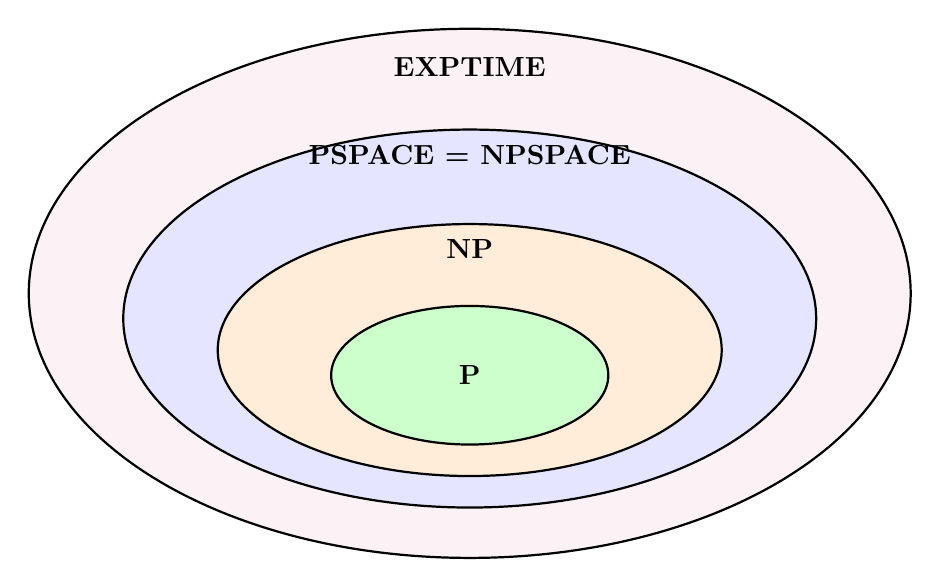
\begin{tikzpicture}[scale=0.8]
    \draw[thick, fill=purple!5] (0,0) ellipse (7cm and 4.2cm);
    \node at (0, 3.6) {\textbf{EXPTIME}};
    \draw[thick, fill=blue!10] (0,-0.4) ellipse (5.5cm and 3.0cm);
    \node at (0, 2.2) {\textbf{PSPACE = NPSPACE}};
    \draw[thick, fill=orange!15] (0,-0.9) ellipse (4.0cm and 2.0cm);
    \node at (0, 0.7) {\textbf{NP}};
    \draw[thick, fill=green!20] (0,-1.3) ellipse (2.2cm and 1.1cm);
    \node at (0, -1.3) {\textbf{P}};
\end{tikzpicture}
\end{center}
\end{solutionbox}

% ==============================================================================
% EXAM 2017-2018
% ==============================================================================
\part{Examination 2017--2018 (07/04/2019)}

\section{Question 9: Logical Bitwise OR Machine}
\begin{questionbox}{Question 9 (2017--18)}
Design a Turing machine (TM) that takes as input two numbers $N_1$ and $N_2$ of equal length in binary and computes the logical OR of the two numbers. The tape initially contains $N_1 \# N_2 \#$, where `\#' is a tape symbol that is used as the separator. Your TM should terminate with the OR of the two numbers in binary after the second \#.
\end{questionbox}

\begin{solutionbox}
\textbf{Solution:} Employs multi-track checkoff logic identical to 2019--20 Q9, outputting $d = a \lor b$:
$$\delta_{\text{OR}}(a, b) = a \lor b = \begin{cases} 0 & \text{if } a=0 \text{ and } b=0 \\ 1 & \text{otherwise} \end{cases}$$

\textbf{Expanded High-Level Flow:}
Using the same multi-track bit-transport architecture, mark each processed bit and store the currently transported bit in the finite control[cite: 2]:
$$[q_0,B]\xrightarrow{\text{read }a}[q_1,a]
\xrightarrow{\text{cross }\#_1}[q_2,a]
\xrightarrow{\text{read }b}[q_3,a\lor b]
\xrightarrow{\text{cross }\#_2}\text{append }(a\lor b)
\xrightarrow{\text{rewind}}[q_0,B]\text{[cite: 2]}.$$
Thus each pair of corresponding bits is processed once and its OR is appended after the second separator.
\end{solutionbox}

\section{Question 10: True/False on TM Simulation}
\begin{questionbox}{Question 10 (2017--18)}
Briefly explain whether the following statements are true or false: \\
(i) A one-tape Turing machine with multiple tracks can simulate a Multi-tape Turing machine[cite: 3]. \\
(ii) A deterministic Turing machine can simulate $n$ moves of a non-deterministic Turing machine in $P(n)$ moves, where $P(n)$ is some polynomial in $n$[cite: 3]. \\
(iii) A deterministic Turing machine can simulate $n$ moves of a conventional computer in $P(n)$ moves, where $P(n)$ is some polynomial in $n$[cite: 3].
\end{questionbox}

\begin{solutionbox}
\textbf{(i) TRUE[cite: 3]:} $2k$ tracks simulate $k$ tapes with $O(n^2)$ quadratic slowdown[cite: 3]. \\
\textbf{(ii) FALSE[cite: 3]:} DTM requires $O(m^n)$ exponential time to simulate breadth-first search of an NTM[cite: 3]. \\
\textbf{(iii) TRUE[cite: 3]:} DTM simulates a computer in $O(n^6)$ polynomial time[cite: 3].
\end{solutionbox}

\section{Question 11: Undecidability Definitions}
\begin{questionbox}{Question 11 (2017--18)}
Define the following: (i) Diagonalization language, (ii) Universal language, (iii) Halting problem. Show that one of the above is not recursively enumerable (RE).
\end{questionbox}

\begin{solutionbox}
\textbf{Solution:} Refer to 2022--23 Question 12 for the full proof showing $L_d$ is not RE via Cantor's diagonal contradiction.
\end{solutionbox}

% ==============================================================================
% EXAM 2016-2017
% ==============================================================================
\part{Examination 2016--2017 (22/02/2018)}

\section{Question 5(b): Binary Number Incrementer ($N \mapsto N+1$)}
\begin{questionbox}{Question 5(b) (2016--17)}
Design a Turing Machine (TM) that takes as input a number $N$ in binary and adds 1 to it. Initially the tape will contain (in its leftmost portion) a $\#$ followed by the number $N$ in binary (e.g., $\#101$), and the tape head will be on $\#$. Your TM should halt after converting the $N$ into $N+1$. You may replace the $\#$ with 0 or 1 if you need.
\end{questionbox}

\begin{solutionbox}
\textbf{Design Logic (Right-to-Left Ripple Carry):}
\begin{enumerate}[leftmargin=*]
    \item \textbf{Scan to the LSB:} Starting on $\#$, move right over the complete binary number until the first blank $B$, then step left onto the least significant bit.
    \item \textbf{Add 1 with a ripple carry:} If the current bit is $0$, rewrite it as $1$ and the carry is finished. If it is $1$, rewrite it as $0$ and continue moving left with the carry.
    \item \textbf{Overflow:} If the carry reaches $\#$, every original bit was $1$. Replace $\#$ by $1$; for example $\#111\rightarrow1000$.
\end{enumerate}

\textbf{1. Transition Rules:}
\begin{align*}
\delta(q_0, \#) &= (q_{\text{seek}}, \#, R) \quad \text{(Scan to LSB)} \\
\delta(q_{\text{seek}}, 0/1) &= (q_{\text{seek}}, 0/1, R) \\
\delta(q_{\text{seek}}, B) &= (q_{\text{add}}, B, L) \quad \text{(Land on LSB)} \\
\delta(q_{\text{add}}, 0) &= (q_{\text{done}}, 1, L) \quad \text{(Carry absorbed!)} \\
\delta(q_{\text{add}}, 1) &= (q_{\text{add}}, 0, L) \quad \text{(Ripple carry continues)} \\
\delta(q_{\text{add}}, \#) &= (q_{\text{halt}}, 1, S) \quad \text{(Overflow: e.g., } \#111 \rightarrow 1000\text{)} \\
\delta(q_{\text{done}}, 0/1) &= (q_{\text{done}}, 0/1, L) \\
\delta(q_{\text{done}}, \#) &= (q_{\text{halt}}, \#, R) \quad \text{(HALT)}
\end{align*}

\textbf{2. Trace for $N=1011_2$ ($11_{10}\rightarrow12_{10}=1100_2$):}
$$
\begin{array}{rll}
q_0\#1011 & \vdash \#q_{\text{seek}}1011 \vdash^* \#1011q_{\text{seek}}B & \text{(Seek to end)}\\
& \vdash \#101q_{\text{add}}1 & \text{(At LSB)}\\
& \vdash \#10q_{\text{add}}0 & (1+1=0\text{ with carry})\\
& \vdash \#1q_{\text{add}}00 & (1+1=0\text{ with carry})\\
& \vdash \#q_{\text{done}}1100 & (0+1=1,\text{ carry resolved})\\
& \vdash q_{\text{done}}\#1100 \vdash \#q_{\text{halt}}1100 & \textbf{(Halt: output is }1100\textbf{)}
\end{array}
$$
\end{solutionbox}

\section{Question 6(c): Unordered Equal Number of 0s and 1s}
\begin{questionbox}{Question 6(c) (2016--17)}
Define a Turing Machine for the set of strings with an equal number of 0's and 1's.
\end{questionbox}

\begin{solutionbox}
\textbf{1. Strategy:}
Repeatedly find the first unmarked $0$, mark it $X$, and find an unmarked $1$ to mark $Y$[cite: 2]. If a $1$ is found first, mark $Y$ and search for a matching $0$ to mark $X$[cite: 2]. If the entire tape is cleanly converted to $X$s and $Y$s without any unpaired symbols, accept[cite: 2].

More explicitly:
\begin{enumerate}[leftmargin=*]
    \item Scan left-to-right for the first unmarked symbol[cite: 2].
    \item If it is $0$, rewrite it as $X$ and search for an unmarked $1$ to rewrite as $Y$[cite: 2].
    \item If it is $1$, rewrite it as $Y$ and search for an unmarked $0$ to rewrite as $X$[cite: 2].
    \item Rewind to the left end and repeat[cite: 2].
    \item Accept if only $X$'s, $Y$'s and blanks remain; reject if one symbol cannot be paired[cite: 2].
\end{enumerate}

\textbf{2. Formal Specification:}
$$M=(\{q_0,q_{\text{find1}},q_{\text{find0}},q_{\text{rewind}},q_{\text{verify}},q_{\text{accept}}\},
\{0,1\},\{0,1,X,Y,B\},\delta,q_0,B,\{q_{\text{accept}}\})\text{[cite: 2]}.$$
\end{solutionbox}

\section{Question 7(a): Connected Graph Decidability}
\begin{questionbox}{Question 7(a) (2016--17)}
Let $A = \{\langle G \rangle \mid G \text{ is a connected undirected graph}\}$. Is it possible to design a Turing Machine that can decide $A$? If yes, briefly discuss your design and demonstrate with a suitable example.
\end{questionbox}

\begin{solutionbox}
\textbf{Yes, $A$ is Decidable.}
A Turing Machine can implement Breadth-First Search (BFS) or Depth-First Search (DFS) on the graph string $\langle G \rangle$:
\begin{enumerate}[leftmargin=*]
    \item Mark the first vertex $v_1$ of $G$ with a dot/marker on the tape.
    \item Repeat until no new nodes can be marked:
    \begin{itemize}
        \item For each marked vertex $u$, scan the edge list of $G$ on the tape.
        \item For every edge $(u, v)$, if $v$ is unmarked, place a mark on $v$.
    \end{itemize}
    \item Scan the node list of $G$. If every vertex has a mark, \textbf{ACCEPT}. Otherwise, \textbf{REJECT}.
\end{enumerate}
Since $|V|$ and $|E|$ are finite, this algorithm halts on all inputs, deciding $A$.
\end{solutionbox}

\section{Question 8(a): Undecidability of $A_{\text{TM}}$}
\begin{questionbox}{Question 8(a) (2016--17)}
Prove that the language $A_{\text{TM}} = \{\langle M, w \rangle \mid M \text{ is a Turing Machine accepting } w\}$ is undecidable.
\end{questionbox}

\begin{solutionbox}
\textbf{Proof by Diagonalization:}
Assume $H$ is a decider for $A_{\text{TM}}$:
$$H(\langle M, w \rangle) = \begin{cases} \text{ACCEPT} & \text{if } M \text{ accepts } w \\ \text{REJECT} & \text{if } M \text{ does not accept } w \end{cases}$$
Construct decider $D$:
``On input $\langle M \rangle$, run $H$ on $\langle M, \langle M \rangle \rangle$. Output the opposite: if $H$ accepts, REJECT; if $H$ rejects, ACCEPT.''

Running $D(\langle D \rangle)$ yields:
$$D \text{ accepts } \langle D \rangle \iff H(\langle D, \langle D \rangle \rangle) \text{ rejects} \iff D \text{ does not accept } \langle D \rangle$$
This contradiction proves that $A_{\text{TM}}$ is \textbf{undecidable}.
\end{solutionbox}

% ==============================================================================
% EXAM 2015-2016
% ==============================================================================
\part{Examination 2015--2016 (25/01/2017)}

\section{Question 7(a): Turing Machine for $\{a^n b^n c^n \mid n \ge 1\}$}
\begin{questionbox}{Question 7(a) (2015--16)}
Design a Turing machine for the language $\{a^n b^n c^n \mid n \ge 1\}$[cite: 5]. Also briefly describe its working principle[cite: 5].
\end{questionbox}

\begin{solutionbox}
\textbf{1. Working Principle:}
\begin{enumerate}[leftmargin=*]
    \item In $q_0$, find the leftmost unmarked $a$, replace it by $X$, and move right[cite: 2].
    \item Skip remaining $a$'s and already marked $Y$'s until the first unmarked $b$ is found; replace that $b$ by $Y$[cite: 2].
    \item Continue right, skipping $b$'s and previously marked $Z$'s, until the first unmarked $c$ is found; replace it by $Z$[cite: 2].
    \item Rewind left to the marked $X$, then begin the next matching round[cite: 2].
    \item When no unmarked $a$ remains, verify that the rest of the input consists only of $Y$'s and $Z$'s. Reaching blank $B$ means accept[cite: 2].
\end{enumerate}
Each round therefore matches exactly one $a$, one $b$, and one $c$.

\textbf{2. State Transition Diagram:}
\begin{center}
\begin{tikzpicture}[->, >=Stealth, auto, node distance=2.6cm, semithick]
    \node[state, initial] (q0) {$q_0$};
    \node[state] (q1) [right of=q0] {$q_1$};
    \node[state] (q2) [right of=q1] {$q_2$};
    \node[state] (q3) [below of=q2] {$q_3$};
    \node[state] (q4) [below of=q0] {$q_4$};
    \node[state, accepting] (qacc) [right of=q4] {$q_{\text{accept}}$};

    \path (q0) edge node[above] {$a/X, R$[cite: 2]} (q1)
               edge node[left] {$Y/Y, R$[cite: 2]} (q4)
          (q1) edge [loop above] node {$a/a, R;\; Y/Y, R$[cite: 2]} (q1)
               edge node[above] {$b/Y, R$[cite: 2]} (q2)
          (q2) edge [loop above] node {$b/b, R;\; Z/Z, R$[cite: 2]} (q2)
               edge node[right] {$c/Z, L$[cite: 2]} (q3)
          (q3) edge [loop below] node[align=center] {$a,b,Y,Z / \\ \text{same}, L$[cite: 2]} (q3)
               edge [bend left=20] node[left] {$X/X, R$[cite: 2]} (q0)
          (q4) edge [loop below] node {$Y/Y, R;\; Z/Z, R$[cite: 2]} (q4)
               edge node[above] {$B/B, R$[cite: 2]} (qacc);
\end{tikzpicture}
\end{center}
\end{solutionbox}

\section{Question 8(a): Monus Variant $\max(b-a, 0)$}
\begin{questionbox}{Question 8(a) (2015--16)}
Design a Turing machine that computes the function $a \dot{-} b = \max(b - a, 0)$[cite: 5]. Initially the tape contains $a$, followed by $b$, represented by consecutive 1's separated by the symbol 0[cite: 5]. After computation, the tape will contain only the output represented by consecutive 1's surrounded by infinite blanks[cite: 5].
\end{questionbox}

\begin{solutionbox}
\textbf{Solution:} Symmetrical to the monus machine in Lecture 4[cite: 2]. Here $1^a 0 1^b$ cancels one $1$ of $a$ on the left and one $1$ of $b$ on the right until $a$ is exhausted[cite: 2]. If $b \ge a$, the remaining $b-a$ ones are kept[cite: 2]. If $a > b$, all symbols are erased to $B$[cite: 2].
\end{solutionbox}

\section{Question 8(b): Multiple Tracks vs. Multiple Tapes}
\begin{questionbox}{Question 8(b) (2015--16)}
Describe how multiple tracks and multiple tapes extend the basic Turing machine[cite: 5]. Briefly discuss the difference between these extensions[cite: 5].
\end{questionbox}

\begin{solutionbox}
\begin{center}
\small
\begin{tabular}{p{7.5cm}p{7.5cm}}
\toprule
\textbf{Multiple Tracks}[cite: 2] & \textbf{Multiple Tapes}[cite: 3] \\
\midrule
Single physical tape head scanning all tracks of cell $i$ simultaneously[cite: 2]. & $k$ independent heads moving independently in different directions[cite: 3]. \\
Tape alphabet is a Cartesian product: $\Gamma = \Gamma_1 \times \dots \times \Gamma_k$[cite: 2]. & Each tape maintains its own separate storage and head cursor[cite: 3]. \\
Requires 0 extra simulation steps ($O(1)$ overhead)[cite: 2]. & Simulating on 1 tape requires quadratic $O(n^2)$ slowdown[cite: 3]. \\
\bottomrule
\end{tabular}
\end{center}
\end{solutionbox}

% ==============================================================================
% EXAM 2013-2014
% ==============================================================================
\part{Examination 2013--2014 (06/08/2015)}

\section{Question 2(a): Deciding $\{0^N 1^N 0^N \mid N \ge 0\}$}
\begin{questionbox}{Question 2(a) (2013--14)}
Build a Turing machine to recognize the language $L = \{0^N 1^N 0^N \mid N \ge 0\}$.
\end{questionbox}

\begin{solutionbox}
\textbf{Solution:} Matches three blocks in lockstep:
$$(q_0, 0) \rightarrow \text{mark } X \xrightarrow{\text{seek } 1} \text{mark } Y \xrightarrow{\text{seek } 0} \text{mark } Z \xrightarrow{\text{rewind to } X} q_0$$
Verify all $0$s, $1$s, and $0$s are matched $\rightarrow$ Accept.
\end{solutionbox}

\section{Question 2(b): Recognizing Left End of the Tape}
\begin{questionbox}{Question 2(b) (2013--14)}
How can we recognize the left end of the tape of a Turing machine? Explain.
\end{questionbox}

\begin{solutionbox}
\textbf{Methods to detect the left end:}
1. \textbf{Special Endmarker Symbol ($\$$):} The machine initializes by shifting input one cell right and writing $\$$ in cell 0. If head reads $\$$, it knows it is at the left boundary.
2. \textbf{Semi-Infinite 2-Track Simulation:} An asterisk $*$ is placed in the lower track of cell 0[cite: 3]. Moving left onto $*$ triggers a track-switch and reversal[cite: 3].
\end{solutionbox}

\section{Question 3(a): Structural TM Properties}
\begin{questionbox}{Question 3(a) (2013--14)}
Answer the following questions and explain your reasoning: \\
(i) Can a Turing machine ever write the blank symbol on its tape? \\
(ii) Can the tape alphabet $\Gamma$ be the same as the input alphabet $\Sigma$? \\
(iii) Can a Turing machine's head ever be in the same location in two successive steps? \\
(iv) Can a Turing machine contain just a single state?
\end{questionbox}

\begin{solutionbox}
\textbf{(i) YES[cite: 2].} The blank symbol $B \in \Gamma$, so $\delta(q, X) = (p, B, D)$ is a legal transition that writes $B$[cite: 2]. \\
\textbf{(ii) NO[cite: 2].} By formal definition, the blank symbol $B \in \Gamma$ but $B \notin \Sigma$[cite: 2]. Hence, $\Sigma \subsetneq \Gamma$ always[cite: 2]. \\
\textbf{(iii) NO in basic model, YES in multitape[cite: 2, 3].} In standard 1-tape formal definition, direction $D \in \{L, R\}$, so head displacement is strictly non-zero[cite: 2]. In multi-tape TMs, stationary move $S$ is explicitly permitted[cite: 3]. \\
\textbf{(iv) YES.} A TM can have $Q = \{q_0\}$ with $F = \{q_0\}$ (accepting $\Sigma^*$ immediately) or $F = \emptyset$ (halting or looping immediately).
\end{solutionbox}

\section{Question 3(b): Decidability of the Mars-Life Language}
\begin{questionbox}{Question 3(b) (2013--14)}
Let $A$ be the language containing only the single string $s$, where:
$$s = \begin{cases} 0 & \text{if life never will be found on Mars} \\ 1 & \text{if life will be found on Mars someday} \end{cases}$$
Is $A$ decidable? Why or why not? Assume the question has an unambiguous YES or NO answer.
\end{questionbox}

\begin{solutionbox}
\textbf{$A$ is Decidable.}
Since the truth is fixed, $s$ is either the single string ``$0$'' or ``$1$'':
\begin{itemize}[leftmargin=*]
    \item If life will never be found, $A = \{0\}$.
    \item If life will be found, $A = \{1\}$.
\end{itemize}
Both $\{0\}$ and $\{1\}$ are finite languages. Every finite language is regular, and every regular language is decidable[cite: 2]. Even though we do not currently know \textit{which} decider is the correct one, a decider for $A$ mathematically exists.
\end{solutionbox}

% ==============================================================================
% EXAM 2012-2013
% ==============================================================================
\part{Examination 2012--2013 (11/01/2015)}

\section{Question 3(b): Deciding $L = \{w-w-w \mid w \in \{a, b\}^*\}$}
\begin{questionbox}{Question 3(b) (2012--13)}
Let $\Sigma = \{-, a, b\}$ and $L = \{w-w-w \mid w \in \{a, b\}^*\}$. Give a high-level description of a Turing machine $M$ that decides $L$. You may assume $M$ has a doubly infinite tape.
\end{questionbox}

\begin{solutionbox}
\textbf{High-Level Algorithm:}
1. Scan input to verify it contains exactly two `$-$' separators, partitioning tape into three blocks: $w_1 - w_2 - w_3$.
2. For each unchecked character of $w_1$:
   \begin{itemize}
       \item Mark it with $*$, store in state register[cite: 2].
       \item Scan past first `$-$' and match corresponding bit of $w_2$, marking with $*$[cite: 2].
       \item Scan past second `$-$' and match corresponding bit of $w_3$, marking with $*$[cite: 2].
       \item Rewind to the next unchecked bit of $w_1$[cite: 2].
   \end{itemize}
3. If all three blocks are checked simultaneously with no leftover characters in any block, \textbf{ACCEPT}; otherwise \textbf{REJECT}[cite: 2].
\end{solutionbox}

\section{Question 3(c): Parity Rewrite Machine}
\begin{questionbox}{Question 3(c) (2012--13)}
Give the state diagram of a Turing machine $M$ that does the following on input string `$\#w$' where $w \in \{0, 1\}^*$ and $n = |w|$. If $n$ is even, $M$ converts $\#w$ to $\#0^n$. If $n$ is odd, $M$ converts $\#w$ to $\#1^n$. The machine enters accept after conversion.
\end{questionbox}

\begin{solutionbox}
\textbf{1. Execution Flow:}
\begin{itemize}[leftmargin=*]
    \item Scan right from $\#$ toggling between state $q_{\text{even}}$ and $q_{\text{odd}}$ on each bit until reaching $B$.
    \item If at blank in $q_{\text{even}}$, sweep left replacing all bits with $0$ until hitting $\#$, then accept.
    \item If at blank in $q_{\text{odd}}$, sweep left replacing all bits with $1$ until hitting $\#$, then accept.
\end{itemize}
\end{solutionbox}

% ==============================================================================
% EXAM 2011-2012
% ==============================================================================
\part{Examination 2011--2012 (22/07/2013)}

\section{Question 1(a): Modified Unary Subtraction}
\begin{questionbox}{Question 1(a) (2011--12)}
Construct the state transition diagram for a Turing machine to compute $f(x, y) = x - y$, where $x \ge y$. Numbers are represented in a modified unary system where integer $N$ is represented by repeating symbol `1' $N+1$ times (e.g., $0 \rightarrow 1, 1 \rightarrow 11, 2 \rightarrow 111$).
\end{questionbox}

\begin{solutionbox}
\textbf{Solution:} Input format: $1^{x+1} 0 1^{y+1}$.
Each subtraction cycle erases one `1' from $x$ on the left and one `1' from $y$ on the right. When $y$ has only a single `1' left (representing $0$), the remaining ones in the first block represent $(x-y)+1$, which is the exact modified unary encoding of $x-y$.
\end{solutionbox}

\section{Question 2(a): 2-Tape Decider for $L = \{w c w^R\}$}
\begin{questionbox}{Question 2(a) (2011--12)}
Construct the state transition diagram of a 2-tape Turing machine to decide $L = \{w c w^R \mid w \in \{a, b\}^*\}$.
\end{questionbox}

\begin{solutionbox}
\textbf{2-Tape Algorithm:}
1. \textbf{Copy Phase:} Read Tape 1, copy $w$ onto Tape 2, moving both heads right until Tape 1 reads $c$.
2. \textbf{Positioning:} Move Tape 1 head one cell right (onto $w^R$). Keep Tape 2 head on the last copied character.
3. \textbf{Mirror Comparison:} Move Tape 1 head right and Tape 2 head left in lockstep:
   $$\text{If } \text{Tape1}[i] == \text{Tape2}[j] \implies \text{continue}$$
4. If both tapes hit blank simultaneously, \textbf{ACCEPT}; if any mismatch occurs, \textbf{REJECT}.
\end{solutionbox}

% ==============================================================================
% EXAM 2008-2009 & 2007-2008
% ==============================================================================
\part{Earlier BUET Papers (2007--2010)}

\section{Exam 2009--2010: Question 12(a) (Double Consecutive `a' Scanner)}
\begin{questionbox}{Question 12(a) (2009--10)}
Write out in full a Turing Machine that scans to the right until it finds two consecutive $a$'s and then halts. Alphabet is $\{a, b, B\}$.
\end{questionbox}

\begin{solutionbox}
$$M = (\{q_0, q_1, q_{\text{halt}}\}, \{a, b\}, \{a, b, B\}, \delta, q_0, B, \{q_{\text{halt}}\}) \text{[cite: 2]}$$
\begin{center}
\small
\begin{tabular}{lll}
\toprule
\textbf{State} & \textbf{Scanned} & \textbf{Transition} \\
\midrule
$q_0$ & $a$ & $(q_1, a, R)$ (First $a$ found!) \\
$q_0$ & $b$ & $(q_0, b, R)$ \\
$q_1$ & $a$ & $(q_{\text{halt}}, a, S)$ (\textbf{Two consecutive $a$'s $\implies$ HALT}) \\
$q_1$ & $b$ & $(q_0, b, R)$ (Reset back to $q_0$) \\
\bottomrule
\end{tabular}
\end{center}
\end{solutionbox}

\section{Exam 2007--2008: Question 7 (Trace of 0011 on $0^n 1^n$ TM)}
\begin{questionbox}{Question 7 (2007--08)}
Design a Turing machine (TM) to decide the language $\{0^n 1^n \mid n \ge 1\}$ and depict it using a transition table[cite: 5]. Show the instantaneous descriptions (ID's) of the TM if the input tape contains 0011[cite: 5].
\end{questionbox}

\begin{solutionbox}
\textbf{Complete ID Trace for $0011$[cite: 2]:}
\begin{align*}
q_0 0011 &\vdash X q_1 011 \vdash X0 q_1 11 \vdash X q_2 0Y1 \vdash q_2 X0Y1 \vdash X q_0 0Y1 \text{[cite: 2]} \\
&\vdash XX q_1 Y1 \vdash XXY q_1 1 \vdash XX q_2 YY \vdash X q_2 XYY \vdash XX q_0 YY \text{[cite: 2]} \\
&\vdash XXY q_3 Y \vdash XXYY q_3 B \vdash XXYYB q_4 B \quad \text{\textbf{(Enters accept state $q_4$)}} \text{[cite: 2]}
\end{align*}
\end{solutionbox}

\section{Exam 2007--2008: Question 10 (Simulating a Computer by a TM)}
\begin{questionbox}{Question 10 (2007--08)}
Describe how a Turing machine can simulate a computer[cite: 5].
\end{questionbox}

\begin{solutionbox}
\textbf{Simulation Architecture (Lecture 6)[cite: 3]:}
The simulation uses a 5-tape Turing Machine[cite: 3]:
\begin{itemize}[leftmargin=*]
    \item \textbf{Tape 1 (RAM):} Formatted as alternating address-value pairs: $\$ 0*w_0 \# 1*w_1 \# 10*w_2 \dots$[cite: 3]
    \item \textbf{Tape 2 (Instruction Counter):} Holds the binary address of the next instruction[cite: 3].
    \item \textbf{Tape 3 (Memory Bus Buffer):} Used to locate and buffer operand addresses and values[cite: 3].
    \item \textbf{Tape 4 (I/O Stream):} Computer's input file[cite: 3].
    \item \textbf{Tape 5 (Scratchpad):} Used to execute ripple-carry additions and shift memory blocks[cite: 3].
\end{itemize}
Each CPU instruction cycle matches the PC on Tape 2 against memory on Tape 1, fetches the opcode and operands to Tape 3, executes the operation (e.g., ALU addition or branching), and increments the PC in $O(n^2)$ time per cycle[cite: 3].
\end{solutionbox}

\end{document}